\chapter{Resultados e Discussão}

Este capítulo apresenta os resultados obtidos durante o desenvolvimento e a avaliação da proposta de solução BURI. O conteúdo encontra-se 
organizado da seguinte forma: primeiramente, aborda-se a análise das respostas de dois questionários aplicados aos alunos sobre o sistema 
de monitoramento na Seção \ref{questionario}. O primeiro questionário foi aplicado na fase de especificação, enquanto o segundo, na etapa de teste de usabilidade. 
Em seguida, realiza-se a avaliação do sistema de alerta na Seção \ref{alerta}, cujas funcionalidades não foram abordadas na etapa anterior. Por fim, apresenta-se na Seção \ref{comparacao} uma análise comparativa 
entre a solução proposta neste trabalho de conclusão de curso e trabalhos acadêmicos de referência.

\section{Análise dos questionários}\label{questionario}

Sobre o primeiro questionário, a primeira pergunta analisada é sobre o preço justo de um dispositivo de medição da qualidade do ar. Do total de 58 entrevistados, 48,3\% 
aceitariam gastar o valor de R\$ 200 até, no máximo, R\$ 500 reais com o protótipo embarcado. Esse dado é um fator positivo do projeto BURI, pois o custo final de montagem do 
protótipo é inferior ao custo da expectativa dos potenciais usuários, totalizando R\$ 146,25 segundo os dados obtidos da Tabela \ref{tabPrecoHardware}.

\begin{figure}[ht]
    \centering
    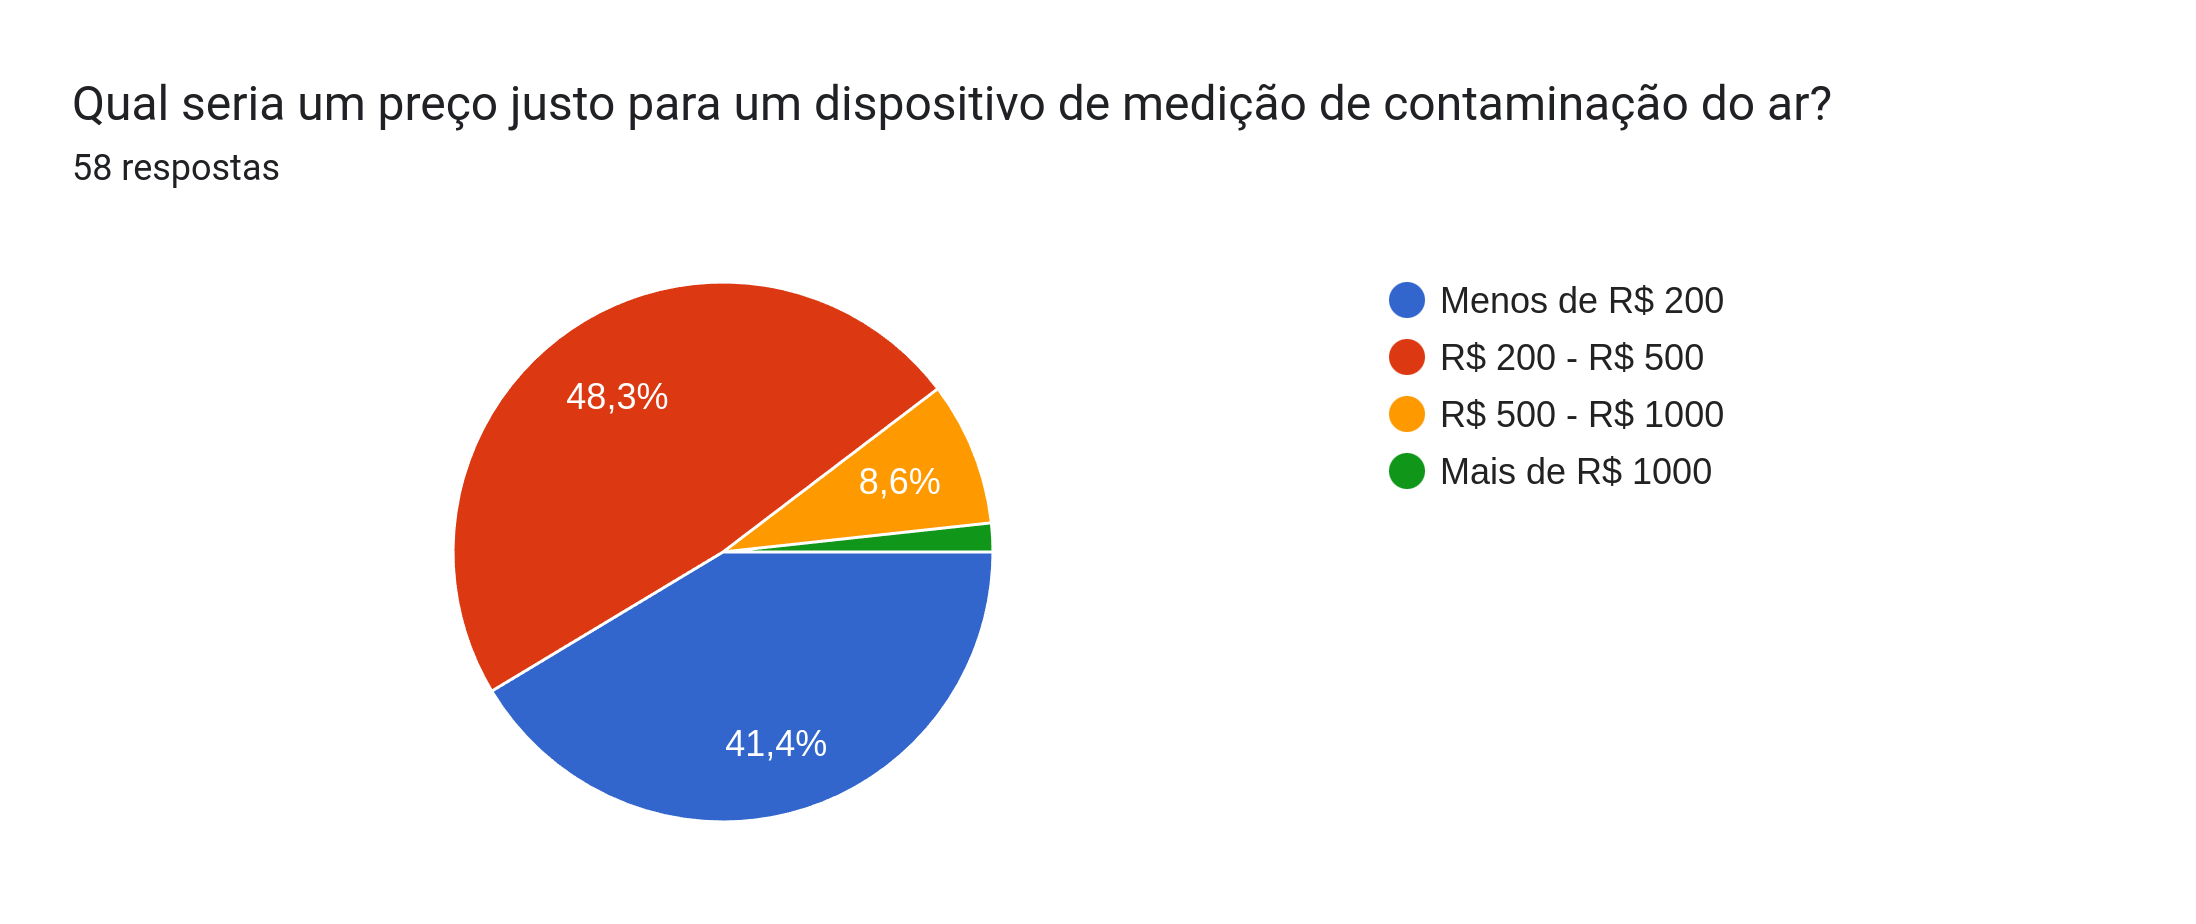
\includegraphics[width=.64\textwidth]{img/questionario/1/graf-preco-hardware.png}
    \caption{Resultado do questionamento sobre o preço justo do dispositivo embarcado de monitoramento da qualidade do ar. Fonte: Autor.}\label{grafPrecoJusto}
\end{figure}

Quanto à frequência de obtenção de dados, a maioria dos usuários optou por receber informações diariamente. No entanto, o dispositivo embarcado realiza a coleta e o envio de dados ao servidor a cada minuto, uma vez 7
que o monitoramento da concentração de monóxido de carbono exige intervalos de coleta curtos devido à gravidade progressiva dos efeitos da intoxicação no organismo. Além disso, o sistema também intervém em situações 
de problemas ambientais, notificando o usuário por meio do aplicativo sobre eventos de risco à saùde.

\begin{figure}[ht]
    \centering
    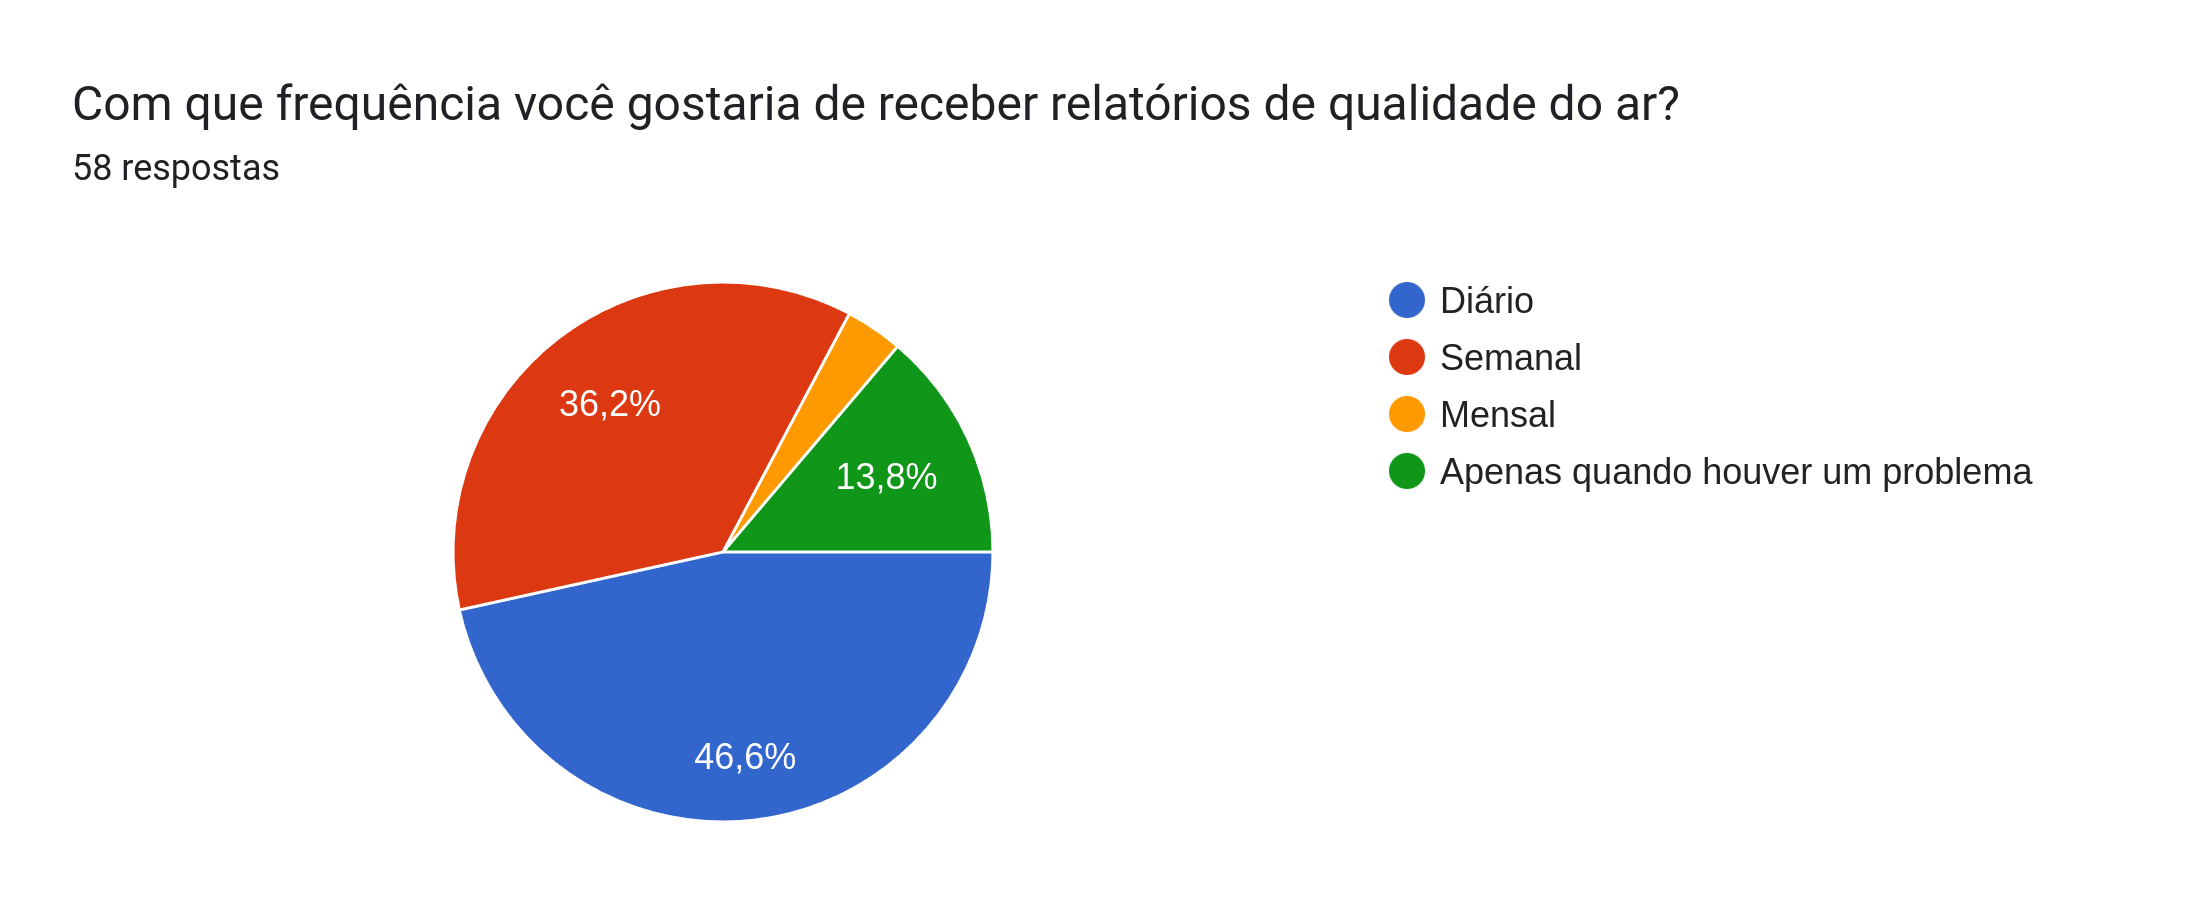
\includegraphics[width=.64\textwidth]{img/questionario/1/graf-info-frequencia.png}
    \caption{Pergunta sobre frequência de coleta de dados e aviso de problema. Fonte: Autor.}\label{grafFrequenciaInfo}
\end{figure}

Para concluir a análise das respostas do primeiro questionário, a pergunta apresentada aos alunos — \textit{``Como você imagina que um dispositivo de medição da contaminação do ar pode melhorar sua qualidade de vida?''} — proporcionou boas motivações. Muitos 
entrevistados mencionaram sintomas respiratórios enfrentados durante períodos de queimadas, ressaltando que um sistema desse tipo seria útil na prevenção dos efeitos nocivos da fumaça para a saúde. O protótipo possui 
relevância informativa, pois permite ao usuário monitorar, em tempo real, as condições ambientais. Contudo, seu papel vai além da mera apresentação de dados, ao fornecer ao dispositivo móvel eventos do ambiente 
acompanhados de descrições detalhadas.

O segundo questionário envolve a execução de tarefas reais com o sistema embarcado. Ao todo, 38 alunos de graduação participaram 
do experimento, com duração média de 30 minutos e grupos formados por duas ou três pessoas. O uso de grupos no teste de usabilidade, e não indivíduos separadamente, é justificado 
pela quantidade grande de participantes e também pela particularidade da tarefa 8, pois sua execução necessita de dois usuários ativos para ocorrer a troca de propriedade. Portanto, 
a Figura x ilustra o resultado geral da execução de atividades descritas na Tabela \ref{tab:cenarios-de-uso}. 

\section{Teste do sistema de alerta}\label{alerta}

\section{Comparação técnica com trabalhos similares}\label{comparacao}